
\chapter{找规律}
\label{chap:pattern}

\section{序列}
\label{sec:series-pattern}

\subsection{基本模式}
\label{sec:basic-patterns-of-sequences}

\begin{example}[等差数列]
  \begin{align*}
    3,\quad 5,\quad 7,\quad 9,\quad 11,\quad ?
  \end{align*}
\end{example}

\begin{example}[等比数列]
  \begin{align*}
    3,\quad 6,\quad 12,\quad 24,\quad 48,\quad 96,\quad ?
  \end{align*}
\end{example}

\begin{example}[双数列]
  \begin{align*}
    1,\quad 2,\quad 3,\quad 4,\quad 5,\quad 8,\quad 7,\quad ?
  \end{align*}
\end{example}
\begin{proof}[提示]\mbox{}\par
  \begin{center}
    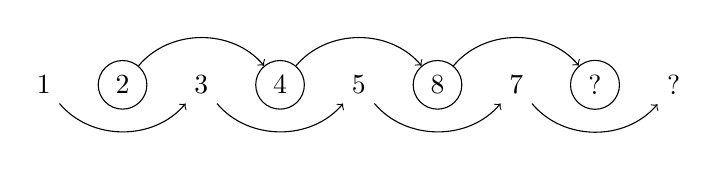
\begin{tikzpicture}[scale=1.0]
      \node(N1) at (1,0) {1};
      \node[draw,circle](N2) at (2,0) {2};
      \node(N3) at (3,0) {3};
      \node[draw,circle](N4) at (4,0) {4};
      \node(N5) at (5,0) {5};
      \node[draw,circle](N8) at (6,0) {8};
      \node(N7) at (7,0) {7};
      \node[draw,circle](N16) at (8,0) {?};
      \node(N9) at (9,0) {?};
      \foreach \x/\y in{N1/N3,N3/N5,N5/N7,N7/N9}{
        \draw[->](\x)edge[bend right=50](\y);
      }
      \foreach \x/\y in{N2/N4,N4/N8,N8/N16}{
        \draw[->](\x)edge[bend left=50](\y);
      }
    \end{tikzpicture}
  \end{center}
  分割成两个数列。
\end{proof}

\begin{example}[双数列]
  \begin{align*}
    8,\quad 14,\quad 10,\quad 12,\quad 12,\quad 9,\quad 14,\quad 5,\quad ?
  \end{align*}
\end{example}
\begin{proof}[提示]\mbox{}\par
  \begin{center}
    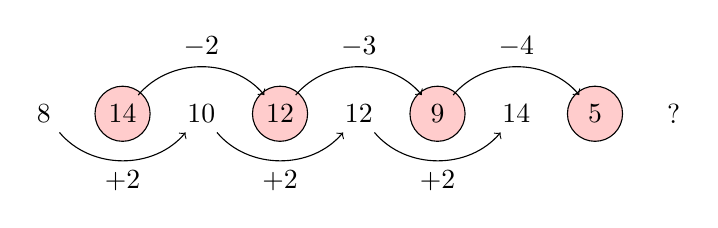
\begin{tikzpicture}[scale=1.0]
      \foreach \x in {2,4,6,8}{
        \draw[fill=red!20](\x,0)circle(.35);
      }
      \foreach \x/\t in{1/8, 2/14, 3/10, 4/12, 5/12, 6/9, 7/14, 8/5, 9/?}{
        \node(N\x) at(\x,0) {\t};
      }
      \foreach \x/\y/\t in{1/3/2, 3/5/2, 5/7/2}{
        \draw[->](N\x)edge[bend right=50]node[below]{$+\t$}(N\y);
      }
      \foreach \x/\y/\t in{2/4/2, 4/6/3, 6/8/4}{
        \draw[->](N\x)edge[bend left=50]node[above]{$-\t$}(N\y);
      }
    \end{tikzpicture}
  \end{center}
  分割成两数列。
\end{proof}

\begin{example}[三数列]
  \begin{align*}
    1,\quad 2,\quad 3,\quad 4,\quad 4,\quad 4,\quad 7,\quad 8,\quad 6,\quad 10,\quad 16,\quad 9,\quad ?
  \end{align*}
\end{example}
\begin{proof}[提示]\mbox{}\par
  \begin{center}
    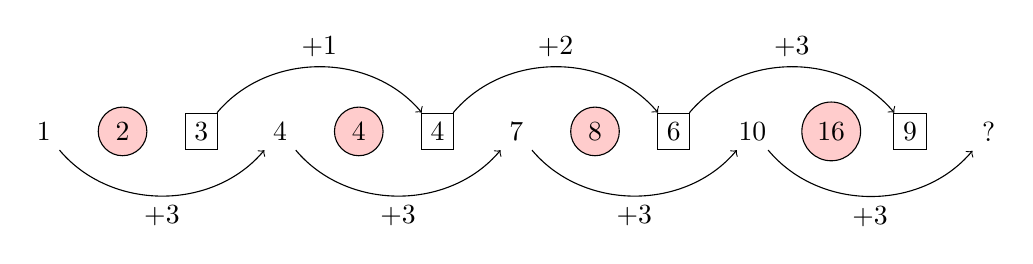
\begin{tikzpicture}[scale=1.0]
      \node(N1) at(1, 0){1};
      \node[draw,circle,fill=red!20](N2) at(2, 0){2};
      \node[draw](N3) at(3, 0){3};
      \node(N4) at(4, 0){4};
      \node[draw,circle,fill=red!20](N5) at(5, 0){4};
      \node[draw](N6) at(6, 0){4};
      \node(N7) at(7, 0){7};
      \node[draw,circle,fill=red!20](N8) at(8, 0){8};
      \node[draw](N9) at(9, 0){6};
      \node(N10)at(10,0){10};
      \node[draw,circle,fill=red!20](N11)at(11,0){16};
      \node[draw](N12)at(12,0){9};
      \node(N13)at(13,0){?};
      \foreach \x/\y in {N1/N4, N4/N7, N7/N10,N10/N13}{
        \draw[->](\x)edge[bend right=50]node[below]{$+3$}(\y);
      }
      \foreach \x/\y/\t in {N3/N6/$+1$, N6/N9/$+2$, N9/N12/$+3$}{
        \draw[->](\x)edge[bend left=50]node[above]{\t}(\y);
      }
    \end{tikzpicture}
  \end{center}
  分割成三个数列。
\end{proof}

\begin{example}[双循环]
  \begin{align*}
    1,\quad 2,\quad 4,\quad 5,\quad 10,\quad 11,\quad 22,\quad 23,\quad 46,\quad ?
  \end{align*}
\end{example}
\begin{proof}[提示]\mbox{}\par
  \begin{center}
    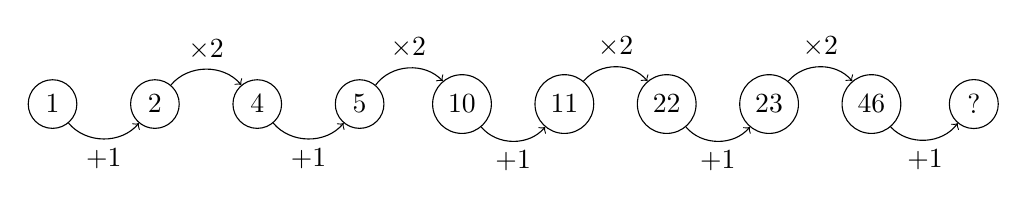
\begin{tikzpicture}[scale=1.0]
      \foreach \x/\y in {1/1, 2/2, 3/4, 4/5, 5/10, 6/11, 7/22, 8/23, 9/46, 10/?}{
        \node[draw,circle](N\x) at(1.3*\x,0) {\y};
      }
      \foreach \x/\y in {N1/N2,N3/N4,N5/N6,N7/N8,N9/N10}{
        \draw[->](\x)edge[bend right=50]node[below]{$+1$}(\y);
      }
      \foreach \x/\y in {N2/N3,N4/N5,N6/N7,N8/N9}{
        \draw[->](\x)edge[bend left=50]node[above]{$\times2$}(\y);
      }
    \end{tikzpicture}
  \end{center}
  以$+1,\ \times2$的模式循环。
\end{proof}

\begin{example}[两级规律]
  \begin{align*}
    1,\quad 3,\quad 7,\quad 15,\quad 31,\quad 63,\quad 127,\quad ?
  \end{align*}
\end{example}
\begin{proof}[提示]通过两级等差等比关系可得。
  \begin{center}
    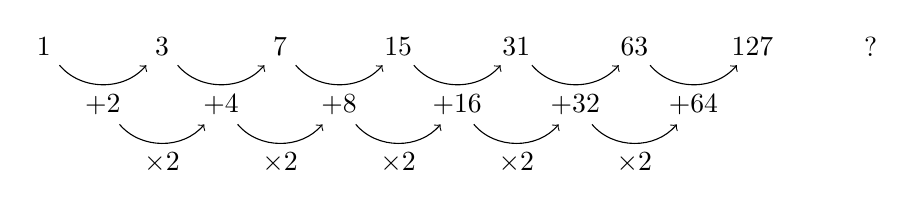
\begin{tikzpicture}[scale=1.0]
      \foreach \x/\y in{1/1, 2/3, 3/7, 4/15, 5/31, 6/63, 7/127, 8/?}{
        \node(N\x) at (1.5*\x, 0) {\y};
      }
      \foreach \x/\y/\t in{1/2/2, 2/3/4, 3/4/8, 4/5/16, 5/6/32, 6/7/64}{
        \draw[->](N\x)edge[bend right=50]node(NN\x)[below]{$+\t$}(N\y);
      }
      \foreach \x/\y in{1/2, 2/3, 3/4,4/5,5/6}{
        \draw[->](NN\x)edge[bend right=50]node[below]{$\times2$}(NN\y);
      }
    \end{tikzpicture}
  \end{center}
  \note 实际上,若熟悉2的各次幂,也容易得到其规律:
  \begin{align*}
    2^0&=1, & 2^1&=2,  & 2^2&=4\\
    2^3&=8, & 2^4&=16, & 2^5&=32\\
    2^6&=64,& 2^7&=128,& 2^8&=256
  \end{align*}
  所以第$n$项的公式为$2^n-1$。
\end{proof}

\begin{example}[三级规律]
  \begin{align*}
    1,\quad 2,\quad 3,\quad 5,\quad 11,\quad 35,\quad ?
  \end{align*}
\end{example}
\begin{proof}[提示]分三层分析。
  \begin{center}
    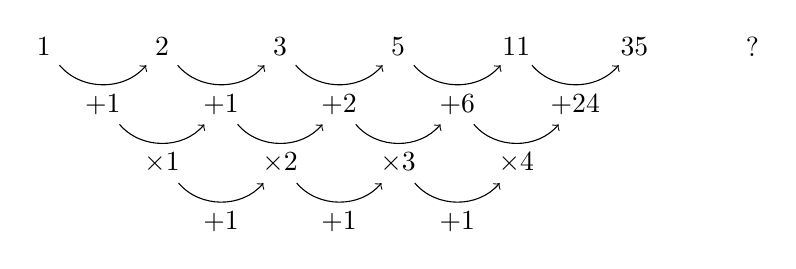
\begin{tikzpicture}[scale=1.0]
      \foreach \x/\y in{1/1, 2/2, 3/3, 4/5, 5/11, 6/35, 7/?}{
        \node(N\x) at (1.5*\x, 0) {\y};
      }
      \foreach \x/\y/\t in{1/2/1, 2/3/1, 3/4/2, 4/5/6, 5/6/24}{
        \draw[->](N\x)edge[bend right=50]node(NN\x)[below]{$+\t$}(N\y);
      }
      \foreach \x/\y/\t in{1/2/1, 2/3/2, 3/4/3, 4/5/4}{
        \draw[->](NN\x)edge[bend right=50]node(NNN\x)[below]{$\times\t$}(NN\y);
      }
      \foreach \x/\y in{1/2,2/3,3/4}{
        \draw[->](NNN\x)edge[bend right=50]node[below]{$+1$}(NNN\y);
      }
    \end{tikzpicture}
  \end{center}
  按此规律,?处应为$35 + 24\times(4+1)=155$。
\end{proof}

\begin{example}[多种规律]\mbox{}\par
  \begin{align*}
    8,\quad 12,\quad 24\quad 60,\quad ?
  \end{align*}
\end{example}
\begin{proof}[提示]
  可以找到两种规律。

  \begin{center}
    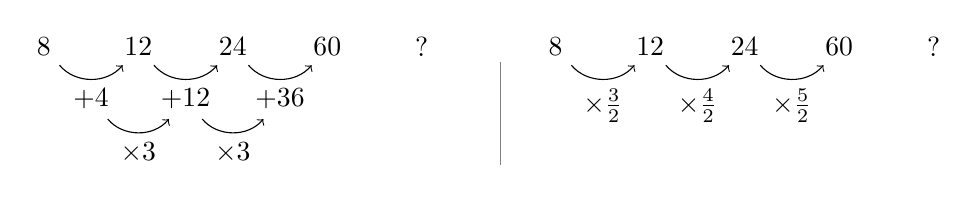
\begin{tikzpicture}[scale=1.0]
      \begin{scope}
        \foreach \x/\t in{1/8, 2/12, 3/24, 4/60, 5/?}{
          \node (N\x) at(1.2*\x,0) {\t};
        }
        \foreach \x/\y/\t in {1/2/4, 2/3/12, 3/4/36}{
          \draw[->](N\x)edge[bend right=50]node(NN\x)[below]{$+\t$}(N\y);
        }
        \foreach \x/\y/\t in {1/2/3, 2/3/3}{
          \draw[->](NN\x)edge[bend right=50]node(NN\x)[below]{$\times\t$}(NN\y);
        }
      \end{scope}
      \begin{scope}[shift={(6.5,0)}]
      \draw[help lines](0.5,-.2)--(0.5,-1.5);
        \foreach \x/\t in{1/8, 2/12, 3/24, 4/60, 5/?}{
          \node (N\x) at(1.2*\x,0) {\t};
        }
        \foreach \x/\y/\t in {1/2/3, 2/3/4, 3/4/5}{
          \draw[->](N\x)edge[bend right=50]node(NN\x)[below]{$\times\frac{\t}{2}$}(N\y);
        }
      \end{scope}
    \end{tikzpicture}
  \end{center}
按这两种规律,可以得到168或者180。至于应该是哪一个,取决于上下文。
\end{proof}

\begin{example}[多种规律]找规律。
  \begin{center}
    \begin{tikzpicture}[scale=1.0]
      \begin{scope}
        \trianglewithfournumbers{5}{8}{3}{18}
      \end{scope}
      \begin{scope}[shift={(3,0)}]
        \trianglewithfournumbers{4}{9}{4}{24}
      \end{scope}
      \begin{scope}[shift={(6,0)}]
        \trianglewithfournumbers{9}{5}{5}{?}
      \end{scope}
    \end{tikzpicture}
  \end{center}
\end{example}
\begin{proof}[提示]可以找到多种规律,应该用哪个取决于上下文。

  \begin{enumerate}
  \item $(\text{左下}-\text{上})\times\text{上}+\text{右下}=\text{中}$.
  \begin{center}
    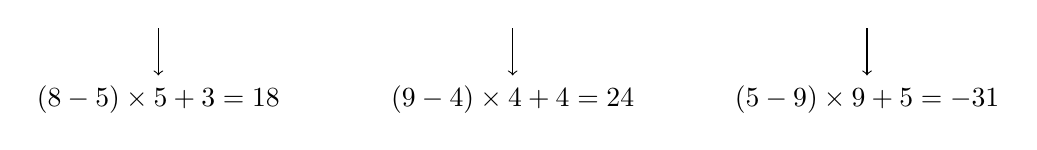
\begin{tikzpicture}[scale=1.0]
      \begin{scope}
        \trianglewithfournumbers{5}{8}{3}{18}
        \draw[->](1,-.2)--(1,-.8);
        \node[below]at(1,-.8){$(8-5)\times5+3=18$};
      \end{scope}
      \begin{scope}[shift={(4.5,0)}]
        \trianglewithfournumbers{4}{9}{4}{24}
        \draw[->](1,-.2)--(1,-.8);
        \node[below]at(1,-.8){$(9-4)\times4+4=24$};
      \end{scope}
      \begin{scope}[shift={(9,0)}]
        \trianglewithfournumbers{9}{5}{5}{?}
        \draw[->](1,-.2)--(1,-.8);
        \node[below]at(1,-.8){$(5-9)\times9+5=-31$};
      \end{scope}
    \end{tikzpicture}
  \end{center}

  \item 分两部分,一是$\underline{\text{上}+\text{左下} + \text{右下}}$,一是$\underline{\text{中}}$.
  \begin{center}
    \begin{tikzpicture}[scale=1.0]
      \begin{scope}
        \trianglewithfournumbers{5}{8}{3}{18}
        \draw[->](1,-.2)--(1,-.8);
        \node[below]at(1,-.8){$5+8+3=16$};
      \end{scope}
      \begin{scope}[shift={(4.5,0)}]
        \trianglewithfournumbers{4}{9}{4}{24}
        \draw[->](1,-.2)--(1,-.8);
        \node[below]at(1,-.8){$4+9+4=17$};
      \end{scope}
      \begin{scope}[shift={(9,0)}]
        \trianglewithfournumbers{9}{5}{5}{?}
        \draw[->](1,-.2)--(1,-.8);
        \node[below]at(1,-.8){$9+5+5=19$};
      \end{scope}
    \end{tikzpicture}
  \end{center}
  \end{enumerate}
  这样分成两部分就变成两个独立的数列:
  \begin{align*}
    \begin{array}{ccc}
    16 & 17 & 19\\
    18 & 24 & ?
    \end{array}
  \end{align*}
  前一个数列$16,17,19$可以尝试套用$+1,+2,\cdots$的模式,后一个数列$18,24,?$信息太少,可以尝试套用等差数列。具体取决于上下文。
\end{proof}


\begin{example}[平方]\mbox{}\par
  \begin{align*}
    2,\quad 3,\quad 7,\quad 45,\quad 2017,\quad ?
  \end{align*}
\end{example}
\begin{proof}[提示]首先可看出来是递增,而且增加的幅度非常快,可以考虑平方、立方等增长速度快的函数。
  \begin{center}
    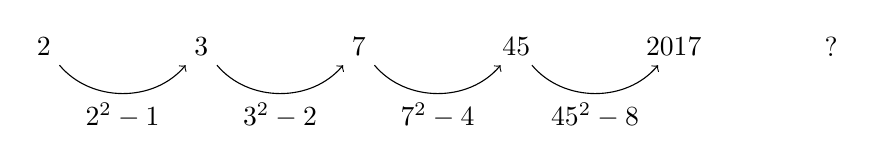
\begin{tikzpicture}[scale=1.0]
      \foreach \x/\t in{1/2, 2/3, 3/7, 4/45, 5/2017, 6/?}{
        \node(N\x) at (2*\x, 0) {\t};
      }
      \foreach \x/\y/\v/\t in{1/2/2/1, 2/3/3/2, 3/4/7/4, 4/5/45/8}{
        \draw[->](N\x)edge[bend right=50]node[below](NN\x){$\v^2-\t$}(N\y);
      }
    \end{tikzpicture}
  \end{center}
  按此规律,下一个应该是$2017^2-16=4068273$。如果有选项,可以简便计算最后一位:
  \begin{align*}
    2017^2-16\equiv 7^2-6\equiv 49-6\equiv3\pmod{10}&\qedhere
  \end{align*}
\end{proof}

\begin{example}
  \begin{align*}
    25,\quad 58,\quad 811,\quad 1114,\quad 1417,\quad ?
  \end{align*}
\end{example}
\begin{proof}[提示]每一项整体来看没有明显关系。将每一项拆开,则可看出其规律。
  \begin{center}
    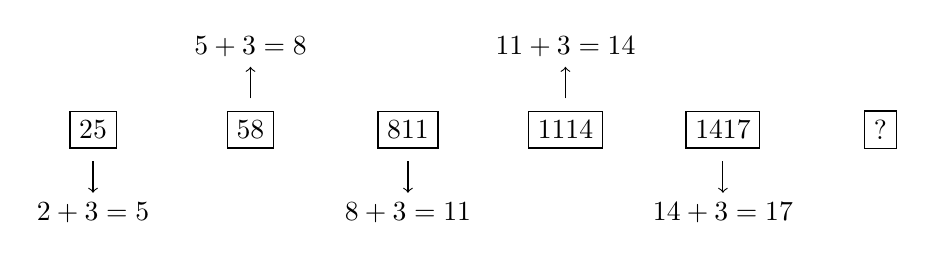
\begin{tikzpicture}[scale=1.0]
      \foreach \x/\t/\v in {1/25/2+3=5,2/58/5+3=8,3/811/8+3=11,4/1114/11+3=14,5/1417/14+3=17,6/?/}{
        \node[draw](N\x)at(2*\x, 0){\t};
        \ifnum\x<6
        \ifodd\x
          \draw[->](2*\x, -.4)--(2*\x, -.8)node[below]{$\v$};
        \else
          \draw[->](2*\x, .4)--(2*\x, .8)node[above]{$\v$};
        \fi\fi
      }
    \end{tikzpicture}
  \end{center}
  按此规律,下一个应该用规律$17+3=20$,即下一个数为$1720$。  
\end{proof}


\begin{example}[单项考虑]\mbox{}\par
  \begin{align*}
    9654,\quad 3248,\quad 5945,\quad 4267,\quad 7963,\quad 1628,\quad 34\underline{\phantom{12}}
  \end{align*}
\end{example}
\begin{proof}[提示]都是四位数,每项之间没有明显的关系。可考虑单独考虑每一项。
  \begin{center}
    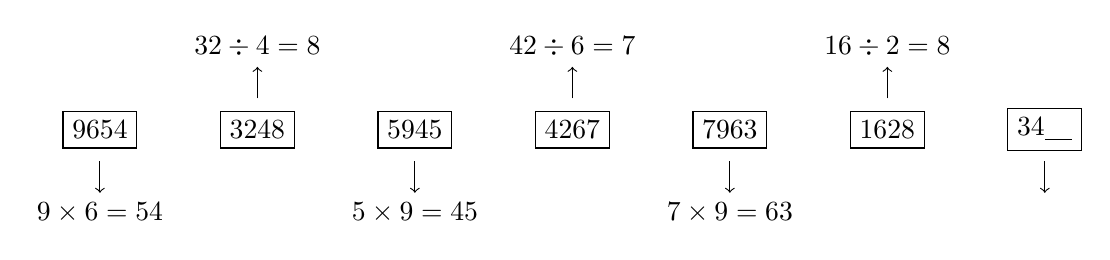
\begin{tikzpicture}[scale=1.0]
      \foreach \x/\t/\u/\v/\w in{1/9654/9/6/54, 2/3248/32/4/8, 3/5945/5/9/45, 4/4267/42/6/7, 5/7963/7/9/63, 6/1628/16/2/8, 7/34\underline{\phantom{12}}//}{
        \node[draw](N\x) at (2*\x, 0){\t};
        \ifnum\x=7
          \draw[->](2*\x, -.4)--(2*\x, -.8);
        \else
          \ifodd\x
            \draw[->](2*\x, -.4)--(2*\x, -.8) node[below]{$\u\times\v=\w$};
          \else
          \draw[->](2*\x, .4)--(2*\x, .8) node[above]{$\u\div\v=\w$};
          \fi
        \fi
      }
    \end{tikzpicture}
  \end{center}
  按此规律,下一个应该是$3\times4=12$,空格处可填$12$。
\end{proof}

\begin{example}[斐波那契数列,Fibonacci sequence]
  \begin{align*}
    1,\quad 1,\quad 2,\quad 3,\quad 5,\quad 8,\quad 13,\quad 21,\quad 34,\quad 55,\quad 89
  \end{align*}
  从第3项起,每项是其前两项的和。
  \begin{center}
    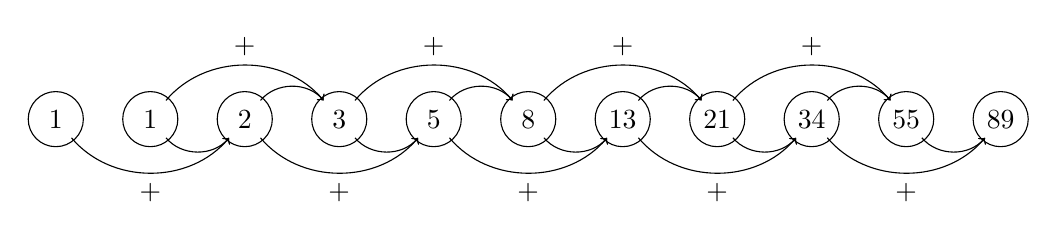
\begin{tikzpicture}[scale=1.0]
      \foreach \x/\t in{1/1, 2/1, 3/2, 4/3, 5/5, 6/8, 7/13, 8/21, 9/34, 10/55, 11/89}{
        \node(N\x) at(1.2*\x, 0) {\t};
        \draw(N\x)circle(.35);
      }
      \foreach \x/\y/\t in {1/3/+,2/3/, 3/5/+,4/5/, 5/7/+,6/7/, 7/9/+,8/9/, 9/11/+,10/11/}{
        \draw[->](N\x)edge[bend right=50]node[below]{$\t$}(N\y);
      }
      \foreach \x/\y/\t in {2/4/+,3/4/, 4/6/+,5/6/, 6/8/+,7/8/, 8/10/+,9/10/}{
        \draw[->](N\x)edge[bend left=50]node[above]{$\t$}(N\y);
      }
    \end{tikzpicture}
  \end{center}
\end{example}


\begin{example}
  \begin{align*}
    1,\quad 3,\quad 4,\quad 8,\quad 16,\quad ?
  \end{align*}
\end{example}
\begin{proof}[提示]与斐波那契数列类似,从第3项起,每项是其前面各项的总和。
  \begin{center}
    \begin{tikzpicture}[scale=1.0]
      \foreach \x/\t/\v in {1/1/, 2/3/, 3/4/4=1+3, 4/8/8=1+3+4, 5/16/16=1+3+4+8, 6/?/}{
        \node[draw](N\x) at (2*\x, 0){\t};
        \ifnum\x>2\ifnum\x<6
        \ifodd\x
          \draw[->](2*\x, -.4)--(2*\x, -.8)node[below]{\small $\v$};
        \else
          \draw[->](2*\x, .4)--(2*\x, .8)node[above]{\small $\v$};
        \fi\fi\fi
      }
    \end{tikzpicture}
  \end{center}
  从而从第4项起,是其前一项的2倍。
\end{proof}


\subsection{外观数列}
\label{sec:look-and-say-sequence}

\begin{example}[外观数列,Look-and-say Sequence,Morris Number Sequence]
  \begin{align*}
    1,\quad 11,\quad 21,\quad 1211,\quad 111221,\quad 312211,\quad 13112221,\quad ?
  \end{align*}
\end{example}
\begin{proof}[说明]
  该序列被称为外观数列,以$1$为开始,后一项是前一项的描述。如第二项$11$是关于第一项$1$的描述,即“$1$个$1$”;第三项$21$是关于第二项$11$的描述,即“$2$个$1$”;第四项$1211$是关于第三项$21$的描述,即“$1$个$2$,$1$个$1$”;第五项$111221$是关于第四项$1211$的描述,即“$1$个$1$,$1$个$2$,$2$个$1$”;以此类推。容易观察到,这个数列里只有数字$1,2,3$。Conway的cosmological theorem里证明了,这个数列邻近两项的比值收敛于一个常数:
  \begin{align*}
    \lim_{n\to\infty}\frac{L_{n+1}}{L_n}=\lambda
  \end{align*}
  此常数$\lambda$称为Conway常数,其值$\lambda\approx 1.303577269034$。

  以$22$开始的外观数列为:
  \begin{align*}
    22,\quad 22,\quad 22,\quad 22,\quad 22,\quad 22,\quad 22,\quad \cdots\cdots
  \end{align*}
  除此之外,以其它数开始的外观数列,都是不会循环的。
\end{proof}

\subsection{有形数}
\label{sec:figurate-number}

\begin{example}[三角形数,Triangular Number]三角形是指按如下方式组成正三角形的\tikz{\draw(0,0)circle(.1);}个数。
  \begin{center}\normalfont
    \begin{tikzpicture}[scale=1.0]
      \foreach \x/\y in{1/1,2/3,3/6,4/10,5/15,6/21,7/28}{
        \begin{scope}[shift={(.3*\y+ .3*\x,0)}]
          \node at(.15*\x+.15,-.5){$\y$};
          \setcounter{X}{0}
          \whiledo{\not{\value{X}>\x}}{%
            \setcounter{Y}{0}
            \whiledo{\value{Y}<\value{X}}{%
              \ifnum\numexpr\x=\theX
                \draw[fill=red!20](.3*\theX - .15*\theY,.3*\theY)circle(.1);
              \else
                \draw(.3*\theX - .15*\theY,.3*\theY)circle(.1);
              \fi
              \stepcounter{Y}
            }
            \stepcounter{X}
          }
        \end{scope}
      }
    \end{tikzpicture}
  \end{center}
  实际上,其通项为
  \begin{align*}
    T_n=1 + 2 + 3 + \cdots + n = \frac{n(n+1)}{2}=\binom{n+1}{2}
  \end{align*}
\end{example}

\begin{example}[平方数,Square Number]与三角形数类似,平方数可以用正方形(Square)描述,如下图。
  \begin{center}
    \begin{tikzpicture}[scale=1.0]
      \foreach \x/\y in{1/1,2/3,3/6,4/10,5/15,6/21,7/28}{
        \begin{scope}[shift={(.3*\y+ .3*\x,0)}]
          \setcounter{X}{\x*\x}
          \node at(.15*\x-.15,-.5){\theX};

          \setcounter{X}{0}
          \whiledo{\value{X}<\x}{%
            \setcounter{Y}{0}
            \whiledo{\value{Y}<\x}{%
              \pgfmathparse{\numexpr\x-1==\theX || \numexpr\x-1==\theY ? int(1):int(0)}
              \ifnum\pgfmathresult>0\relax
                \draw[fill=red!20](.3*\theX, .3*\theY)circle(.1);
              \else
                \draw(.3*\theX, .3*\theY)circle(.1);
              \fi
              \stepcounter{Y}
            }
            \stepcounter{X}
          }
        \end{scope}
      }
    \end{tikzpicture}
  \end{center}
\end{example}

可以注意到,$36$既是正方形数(平方数),也是三角形数。类似的,也可以构造五边形数、六边形数。有趣的是,任意一个六边形数都是三角形数。

\begin{example}[六边形数,Hexagonal Number]\mbox{}\par
  \begin{center}
    \begin{tikzpicture}[scale=1.0]
      \begin{scope}[shift={(0,0)}]
        \draw[fill=red!20](0,0)circle(.1);
        \node at(0,-.5){1};
      \end{scope}
      \begin{scope}[shift={(1,0)}]
        \coordinate (O) at(60:.3);
        \foreach \r in{0.3}{
          \draw($(O)+(0:\r)$)--($(O)+(60:\r)$)--($(O)+(120:\r)$)--($(O)+(180:\r)$)--($(O)+(240:\r)$)--($(O)+(300:\r)$)--cycle;
        }
        \draw[fill=white](0,0)circle(.1);
        \foreach \t in{-60,0,60,120,180}{
          \draw[fill=red!20]($(O)+(\t:.3)$)circle(.1);
        }
        \node at(.15,-.5){6};
      \end{scope}
      \begin{scope}[shift={(2.5,0)}]
        \coordinate (O) at(60:.3);
        \coordinate (O1) at(60:.6);
        \draw($(O1)+(0:.6)$)--($(O1)+(60:.6)$)--($(O1)+(120:.6)$)--($(O1)+(180:.6)$)--($(O1)+(240:.6)$)--($(O1)+(300:.6)$)--cycle;
        \draw($(O)+(-60:.3)$)--($(O)+(0:.3)$)--($(O)+(60:.3)$)--($(O)+(120:.3)$)--($(O)+(180:.3)$);
        \foreach \t in{-120,-60,0,60,120,180}{
          \draw[fill=white]($(O)+(\t:.3)$)circle(.1);
        }
        \coordinate (O) at (60:.6);
        \foreach \x/\t in{1/-60,2/0,3/60,4/120,5/180}{
          \draw[fill=red!20]($(O)+(\t:.6)$)node(N\x){}circle(.1);
        }
        \foreach \x/\y in {1/2, 2/3, 3/4, 4/5}{
          \draw[fill=red!20]($.5*(N\x)+.5*(N\y)$)circle(.1);
        }
        \node at(.3,-.5){15};
      \end{scope}
      \begin{scope}[shift={(4.8,0)}]
        \coordinate (O) at(60:.3);
        \coordinate (O1) at(60:.6);
        \coordinate (O2) at(60:.9);
        \draw($(O2)+(0:.9)$)--($(O2)+(60:.9)$)--($(O2)+(120:.9)$)--($(O2)+(180:.9)$)--($(O2)+(240:.9)$)--($(O2)+(300:.9)$)--cycle;
        \draw($(O1)+(-60:.6)$)--($(O1)+(0:.6)$)--($(O1)+(60:.6)$)--($(O1)+(120:.6)$)--($(O1)+(180:.6)$);
        \draw($(O)+(-60:.3)$)--($(O)+(0:.3)$)--($(O)+(60:.3)$)--($(O)+(120:.3)$)--($(O)+(180:.3)$);
        \foreach \t in{-120,-60,0,60,120,180}{
          \draw[fill=white]($(O)+(\t:.3)$)circle(.1);
        }
        \coordinate (O) at (60:.6);
        \foreach \x/\t in{1/-60,2/0,3/60,4/120,5/180}{
          \draw[fill=white]($(O)+(\t:.6)$)node(N\x){}circle(.1);
        }
        \foreach \x/\y in {1/2, 2/3, 3/4, 4/5}{
          \draw[fill=white]($.5*(N\x)+.5*(N\y)$)circle(.1);
        }

        % new and fill
        \coordinate (O) at (60:.9);
        \foreach \x/\t in{1/-60,2/0,3/60,4/120,5/180}{
          \draw[fill=red!20]($(O)+(\t:.9)$)node(NN\x){}circle(.1);
        }
        \foreach \x/\y in {1/2,2/3,3/4,4/5}{
          \draw[fill=red!20]($1/3*(NN\x)+2/3*(NN\y)$)circle(.1);
          \draw[fill=red!20]($2/3*(NN\x)+1/3*(NN\y)$)circle(.1);
        }
        \node at(.45,-.5){28};
      \end{scope}
    \end{tikzpicture}
  \end{center}
\end{example}

如果把六边形数中间缺的\tikz\draw(0,0)circle(.1);补上,可以得到下图:
\begin{center}
  \begin{tikzpicture}[scale=2.0]
    \coordinate (O1) at (60:.3);
    \coordinate (O2) at (60:.6);
    \coordinate (O3) at (60:.9);
    \coordinate (O4) at (60:1.2);
    \coordinate (V) at ($(O1)+(-120:.3)$);
    \foreach \x/\y/\t/\r in {%
      1/1/-60/.3,  1/2/0/.3,  1/3/60/.3,  1/4/120/.3,  1/5/180/.3,
      2/1/-60/.6,  2/2/0/.6,  2/3/60/.6,  2/4/120/.6,  2/5/180/.6,
      3/1/-60/.9,  3/2/0/.9,  3/3/60/.9,  3/4/120/.9,  3/5/180/.9,
      4/1/-60/1.2, 4/2/0/1.2, 4/3/60/1.2, 4/4/120/1.2, 4/5/180/1.2%
    }{
      \coordinate (V\x\y) at ($(O\x)+(\t:\r)$);
    }
    \draw(V)--(V41)--(V42)--(V43)--(V44)--(V45)--cycle;
    \foreach \x in {1,2,3}{
      \draw(V\x1)--(V\x2)--(V\x3)--(V\x4)--(V\x5);
    }    
    \draw[fill=blue!20](V)circle(.1);
    \foreach \x/\c in{1/red!20,2/blue!20,3/red!20,4/blue!20}{
      \foreach \y in {1,2,3,4,5}{
        \draw[fill=\c](V\x\y)circle(.1);
      }
    }
    \foreach \x in {1,3}{
      \foreach \y in {1,2,3,4,5}{
        \fill[pattern=north west lines, pattern color=black](V\x\y)circle(.1);
      }
    }
    \foreach \x/\y in{1/2,2/3,3/4,4/5}{
      \draw[fill=blue!20]($.5*(V2\x)+.5*(V2\y)$)circle(.1);

      \draw[fill=red!20]($2/3*(V3\x)+1/3*(V3\y)$)circle(.1);
      \draw[fill=red!20]($1/3*(V3\x)+2/3*(V3\y)$)circle(.1);
      \fill[pattern=north west lines,pattern color=black]($2/3*(V3\x)+1/3*(V3\y)$)circle(.1);
      \fill[pattern=north west lines,pattern color=black]($1/3*(V3\x)+2/3*(V3\y)$)circle(.1);

      \draw[fill=blue!20]($.25*(V4\x)+.75*(V4\y)$)circle(.1);
      \draw[fill=blue!20]($.50*(V4\x)+.50*(V4\y)$)circle(.1);
      \draw[fill=blue!20]($.75*(V4\x)+.25*(V4\y)$)circle(.1);
    }
    
    \draw[dashed](O1)circle(.1);
    \draw[dashed]($(V13)+(.3,0)$)circle(.1);

    \coordinate (VV1) at ($.5*(V23)+.5*(V33)$);
    \coordinate (VV2) at ($.5*(V33)+.5*(V43)$);
    \foreach \V/\x in {V35/.6, V35/.9, V35/1.5,
      V23/.3, V23/.9,
      V33/.3,
      VV1/0, VV1/-.3, VV1/-.6, VV1/.6,
      VV2/0, VV2/-.3, VV2/-.6,VV2/-.9
    }{
      \draw[dashed]($(\V)+(\x,0)$)circle(.1);
    }
    \node at(.6,-.3){45};
  \end{tikzpicture}
\end{center}

由递推关系及初始值:
\begin{align*}
  h_{n} = h_{n-1} + 4\times n - 3 = h_{n-1} + 4(n-1) + 1, \quad\quad h_1=1
\end{align*}
其中$4\times n$是因为增加了4条边,每条边的长度为$n$;$-3$是因为其中有3个顶点是共用的。可以得到通项公式
\begin{align*}
  h_{n} & = 1 + (4\times 1 + 1) + (4\times 2 + 1) + \cdots + (4\times (n-1)+1)\\
        & = 1 + (n-1) + 4\left(1+2+3+\cdots + (n-1)\right)\\
        & = n + 4\times\frac{n(n-1)}{2} = n + 2n(n-1) =2n^2-n
\end{align*}


\begin{example}[五角形数,五边形数,Pentagonal Number]\mbox{}\par
  \begin{center}
    \begin{tikzpicture}[scale=1.0]
      \begin{scope}[shift={(0,0)}]
        \draw[fill=red!20](0,0)circle(.1);
        \node at(0,-.5) {1};
      \end{scope}
      \begin{scope}[shift={(1,0)}]
        \node at(.15,-.5) {5};
        \coordinate (O1) at (54:.3);
        \coordinate (V) at (0,0);
        \foreach \x/\y/\t/\r in {1/1/-54/.3, 1/2/18/.3, 1/3/90/.3, 1/4/162/.3}{
          \coordinate(V\x\y) at ($(O\x) + (\t:\r)$);
        }
        \draw(V)--(V11)--(V12)--(V13)--(V14)--cycle;
        \draw[fill=white](V)circle(.1);
        \foreach \x in {1,2,3,4}{
          \draw[fill=red!20](V1\x)circle(.1);
        }
      \end{scope}
      \begin{scope}[shift={(2.8,0)}]
        \node at(.3,-.5) {12};
        \coordinate (O1) at (54:.3);
        \coordinate (O2) at (54:.6);
        \coordinate (V) at (0,0);
        \foreach \x/\y/\t/\r in {1/1/-54/.3, 1/2/18/.3, 1/3/90/.3, 1/4/162/.3,
          2/1/-54/.6, 2/2/18/.6, 2/3/90/.6, 2/4/162/.6
        }{
          \coordinate(V\x\y) at ($(O\x) + (\t:\r)$);
        }
        \draw(V11)--(V12)--(V13)--(V14);
        \draw(V)--(V21)--(V22)--(V23)--(V24)--cycle;
        \draw[fill=white](V)circle(.1);
        \foreach \x in {1,2,3,4}{
          \draw[fill=white](V1\x)circle(.1);
        }
        \foreach \x in {1,2,3,4}{
          \draw[fill=red!20](V2\x)circle(.1);
        }
        \foreach \x/\y in {1/2,2/3,3/4}{
          \draw[fill=red!20]($.5*(V2\x)+.5*(V2\y)$)circle(.1);
        }
      \end{scope}
      \begin{scope}[shift={(5.2,0)}]
        \node at(.5,-.5) {22};
        \coordinate (O1) at (54:.3);
        \coordinate (O2) at (54:.6);
        \coordinate (O3) at (54:.9);
        \coordinate (V) at (0,0);
        \foreach \x/\y/\t/\r in {1/1/-54/.3, 1/2/18/.3, 1/3/90/.3, 1/4/162/.3,
          2/1/-54/.6, 2/2/18/.6, 2/3/90/.6, 2/4/162/.6,
          3/1/-54/.9, 3/2/18/.9, 3/3/90/.9, 3/4/162/.9
        }{
          \coordinate(V\x\y) at ($(O\x) + (\t:\r)$);
        }
        \draw(V11)--(V12)--(V13)--(V14);
        \draw(V21)--(V22)--(V23)--(V24);
        \draw(V)--(V31)--(V32)--(V33)--(V34)--cycle;
        \draw[fill=white](V)circle(.1);
        \foreach \x in {1,2,3,4}{
          \draw[fill=white](V1\x)circle(.1);
        }
        \foreach \x in {1,2,3,4}{
          \draw[fill=white](V2\x)circle(.1);
          \draw[fill=red!20](V3\x)circle(.1);
        }
        \foreach \x/\y in {1/2,2/3,3/4}{
          \draw[fill=white]($.5*(V2\x)+.5*(V2\y)$)circle(.1);

          \draw[fill=red!20]($1/3*(V3\x)+2/3*(V3\y)$)circle(.1);
          \draw[fill=red!20]($2/3*(V3\x)+1/3*(V3\y)$)circle(.1);
        }
      \end{scope}
      \begin{scope}[shift={(8,0)}]
        \node at(.7,-.5) {35};
        \coordinate (O1) at (54:.3);
        \coordinate (O2) at (54:.6);
        \coordinate (O3) at (54:.9);
        \coordinate (O4) at (54:1.2);
        \coordinate (V) at (0,0);
        \foreach \x/\y/\t/\r in {1/1/-54/.3, 1/2/18/.3, 1/3/90/.3, 1/4/162/.3,
          2/1/-54/.6, 2/2/18/.6, 2/3/90/.6, 2/4/162/.6,
          3/1/-54/.9, 3/2/18/.9, 3/3/90/.9, 3/4/162/.9,
          4/1/-54/1.2, 4/2/18/1.2, 4/3/90/1.2, 4/4/162/1.2
        }{
          \coordinate(V\x\y) at ($(O\x) + (\t:\r)$);
        }
        \draw(V11)--(V12)--(V13)--(V14);
        \draw(V21)--(V22)--(V23)--(V24);
        \draw(V31)--(V32)--(V33)--(V34);
        \draw(V)--(V41)--(V42)--(V43)--(V44)--cycle;
        \draw[fill=white](V)circle(.1);
        \foreach \x in {1,2,3,4}{
          \draw[fill=white](V1\x)circle(.1);
        }
        \foreach \x in {1,2,3,4}{
          \draw[fill=white](V2\x)circle(.1);
          \draw[fill=white](V3\x)circle(.1);
          \draw[fill=red!20](V4\x)circle(.1);
        }
        \foreach \x/\y in {1/2,2/3,3/4}{
          \draw[fill=white]($.5*(V2\x)+.5*(V2\y)$)circle(.1);

          \draw[fill=white]($1/3*(V3\x)+2/3*(V3\y)$)circle(.1);
          \draw[fill=white]($2/3*(V3\x)+1/3*(V3\y)$)circle(.1);

          \draw[fill=red!20]($.25*(V4\x)+.75*(V4\y)$)circle(.1);
          \draw[fill=red!20]($.50*(V4\x)+.50*(V4\y)$)circle(.1);
          \draw[fill=red!20]($.75*(V4\x)+.25*(V4\y)$)circle(.1);
        }
      \end{scope}
    \end{tikzpicture}
  \end{center}
\end{example}

五角形数的递推关系是
\begin{align*}
  h_n = h_{n-1} + 3n - 2 = h_{n-1} + 3(n-1) + 1
\end{align*}
从而其通项是
\begin{align*}
  h_n & = 1 + (3\times 1 + 1) + (3\times 2 + 1) + \cdots + (3\times (n-1) + 1) \\
      & = n + 3\left(1 + 2 + \cdots + (n-1)\right)\\
      & = n + 3\times\frac{n(n-1)}{2} = \frac{3n^2-n}{2}
\end{align*}

三角形数、正方形数、五边形数和六边形数等都是{\kai 多边形数},也是{\kai 有形数}。有形数是毕达哥拉斯学派的关注重点之一,是指可以排成一定规律的数。

\subsection{其它}
\label{sec:misc-series}

\begin{example}
  找规律填空:
  \begin{align*}
    1=&5\\
    2=&15\\
    3=&215\\
    4=&3215\\
    5=&??
  \end{align*}
\end{example}
\begin{proof}[提示]
  显然此处$=$不是相等的意思,把$=$号及末尾的$5$去掉,规律就很明显了。
\end{proof}
  
\section{图形}
\label{sec:graph-pattern}

\begin{example}找规律。
  \begin{center}
    \begin{tikzpicture}[scale=1.0]
      % \begin{scope}[shift={(0,0)}]
      %   \coordinate(A) at (0,0);
      %   \coordinate(B) at (2,0);
      %   \coordinate(C) at (60:2);
      %   \coordinate(O) at ($1/3*(A)+1/3*(B)+1/3*(C)$);
      %   \draw(A)--(B)--(C)--cycle;
      %   \node at ($(90:.5)+(O)$) {1};
      %   \node at ($(210:.5)+(O)$) {2};
      %   \node at ($(330:.5)+(O)$) {3};
      % \end{scope}

      \begin{scope}[shift={(3,0)}]
        \coordinate(A) at (0,0);
        \coordinate(B) at (2,0);
        \coordinate(C) at (60:2);
        \coordinate(O) at ($1/3*(A)+1/3*(B)+1/3*(C)$);
        \draw(A)--(B)--(C)--cycle;
        \node at ($(90:.5)+(O)$) {1};
        \node at ($(210:.5)+(O)$) {2};
        \node at ($(330:.5)+(O)$) {3};
      \end{scope}

      \begin{scope}[shift={(6,0)}]
        \coordinate(A) at (0,0);
        \coordinate(B) at (2,0);
        \coordinate(C) at (60:2);
        \coordinate(O) at ($1/3*(A)+1/3*(B)+1/3*(C)$);
        \draw(A)--(B)--(C)--cycle;
        \node at ($(90:.5)+(O)$) {4};
        \node at ($(210:.5)+(O)$) {5};
        \node at ($(330:.5)+(O)$) {6};
      \end{scope}

      \begin{scope}[shift={(9,0)}]
        \coordinate(A) at (0,0);
        \coordinate(B) at (2,0);
        \coordinate(C) at (60:2);
        \coordinate(O) at ($1/3*(A)+1/3*(B)+1/3*(C)$);
        \draw(A)--(B)--(C)--cycle;
        \node at ($(90:.5)+(O)$) {7};
        \node at ($(210:.5)+(O)$) {8};
        \node at ($(330:.5)+(O)$) {9};
      \end{scope}
      
      \begin{scope}[shift={(12,0)}]
        \coordinate(A) at (0,0);
        \coordinate(B) at (2,0);
        \coordinate(C) at (60:2);
        \coordinate(O) at ($1/3*(A)+1/3*(B)+1/3*(C)$);
        \draw(A)--(B)--(C)--cycle;
        \node at ($(90:.5)+(O)$) {10};
        \node at ($(210:.5)+(O)$) {18};
        \node at ($(330:.5)+(O)$) {?};
      \end{scope}
    \end{tikzpicture}
  \end{center}
  \begin{align*}
    (\mathrm{A})\ 200 \quad\quad (\mathrm{B})\ 600 \quad\quad (\mathrm{C})\ 800\quad\quad (\mathrm{D})\ 1200
  \end{align*}
\end{example}
\begin{proof}[提示]平方和之后求数字和,直到最后是一位数。
  \begin{align*}
    &1^2+2^2+3^2 = 14, && \implies 1 + 4 = 5\\
    &4^2+5^2+6^2 = 74, && \implies 7 + 4 = 14, && \implies 1+4=5\\
    &7^2+8^2+9^2 = 194,&& \implies 1+9+4=14, && \implies 1+4=5
  \end{align*}
  按这个规律,?号处填200,最后会得到5。

  \note 对这种规律,知道就知道,不知道也没必要强求,不要钻了牛角尖。非要编的话,比这种更隐晦的规律都有。
\end{proof}


\begin{example}找规律。
  \begin{center}
    \begin{tikzpicture}[scale=1.2]
      \begin{scope}[shift={(0,0)}]
        \trianglewithfournumbers{2}{3}{5}{10}
      \end{scope}
      \begin{scope}[shift={(3,0)}]
        \trianglewithfournumbers{6}{1}{4}{11}
      \end{scope}
      \begin{scope}[shift={(6,0)}]
        \trianglewithfournumbers{3}{7}{?}{15}
      \end{scope}
      \begin{scope}[shift={(9,0)}]
        \trianglewithfournumbers{4}{8}{2}{?}
      \end{scope}
    \end{tikzpicture}
  \end{center}
\end{example}
\begin{proof}[提示]
  每个图中,中间三角形数字是其余三个三角形数字之和。
\end{proof}

\begin{example}找规律。
  \begin{center}
    \begin{tikzpicture}[scale=1.2]
      \begin{scope}[shift={(0,0)}]
        \trianglewithfournumbers{2}{10}{7}{24}
      \end{scope}
      \begin{scope}[shift={(3,0)}]
        \trianglewithfournumbers{3}{6}{5}{21}
      \end{scope}
      \begin{scope}[shift={(6,0)}]
        \trianglewithfournumbers{4}{5}{6}{}
      \end{scope}
    \end{tikzpicture}
  \end{center}
\end{example}
\begin{proof}[提示]
  每个图中,两数的积再加第三个,其和等于中间的数。
\end{proof}

\begin{example}找规律填空。
  \begin{center}
    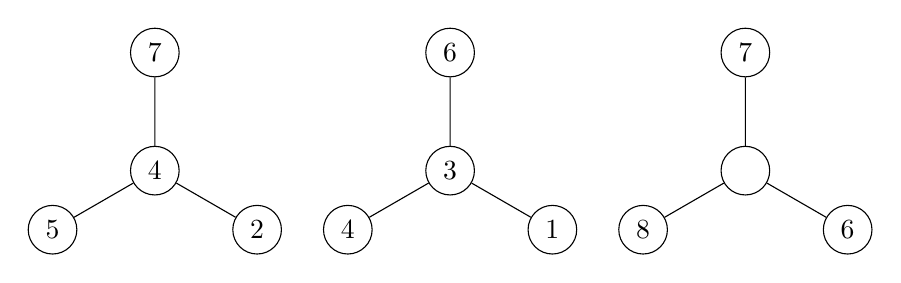
\begin{tikzpicture}[scale=.75]
      \begin{scope}[shift={(0,0)}]
        \node[draw,circle](O) at (0,0)  {4};
        \node[draw,circle](A) at (90:2) {7};
        \node[draw,circle](B) at (210:2){5};
        \node[draw,circle](C) at (330:2){2};
        \draw (O)--(A) (O)--(B) (O)--(C);
      \end{scope}
      \begin{scope}[shift={(5,0)}]
        \node[draw,circle](O) at (0,0)  {3};
        \node[draw,circle](A) at (90:2) {6};
        \node[draw,circle](B) at (210:2){4};
        \node[draw,circle](C) at (330:2){1};
        \draw (O)--(A) (O)--(B) (O)--(C);
      \end{scope}
      \begin{scope}[shift={(10,0)}]
        \node[draw,circle](O) at (0,0)  {\phantom{0}};
        \node[draw,circle](A) at (90:2) {7};
        \node[draw,circle](B) at (210:2){8};
        \node[draw,circle](C) at (330:2){6};
        \draw (O)--(A) (O)--(B) (O)--(C);
      \end{scope}
    \end{tikzpicture}
  \end{center}
\end{example}
\begin{proof}[提示]
  每个图里的4个数分成两组,每组的和相等。
\end{proof}

\begin{example}找规律填空。
  \begin{center}
    \newcommand{\envelopewithfournumbers}[4]{
      \coordinate(A) at (0,0);
      \coordinate(B) at (3,0);
      \coordinate(C) at (3,2);
      \coordinate(D) at (0,2);
      \coordinate(E) at (1.5,.8);
      \coordinate(F) at ($.4*(D)+.6*(E)$);
      \coordinate(G) at ($.4*(C)+.6*(E)$);
      \draw(A)--(B)--(C)--(D)--cycle;
      \draw(D)--(E)--(C) (A)--(F) (B)--(G);
      \node at ($1/3*(D)+1/3*(E)+1/3*(C)$) {#1};
      \node at ($1/3*(A)+1/3*(D)+1/3*(F)$) {#2};
      \node at ($1/3*(B)+1/3*(C)+1/3*(G)$) {#3};
      \node at ($.25*(A)+.5*(E)+.25*(B)$) {#4};
    }
    \begin{tikzpicture}[scale=.75]
      \begin{scope}[shift={(0,0)}]
        \envelopewithfournumbers{8}{2}{4}{6};
      \end{scope}
      \begin{scope}[shift={(4,0)}]
        \envelopewithfournumbers{19}{3}{5}{8};
      \end{scope}
      \begin{scope}[shift={(8,0)}]
        \envelopewithfournumbers{}{4}{6}{10};
      \end{scope}
    \end{tikzpicture}
  \end{center}
\end{example}
\begin{proof}[提示]
  两数的乘积等于另外两数的和。
\end{proof}

\begin{example}找规律填空。
  \begin{center}
    \begin{tikzpicture}[scale=1.5]
      \foreach \dx/\dy/\v in {%
        0/0/2, 1/0/3, 2/0/4, 3/0/15, 4/0/12,
        0/1/3, 1/1/4, 2/1/5, 3/1/28, 4/1/20,
        0/2/4, 1/2/5, 2/2/6, 3/2/46, 4/2/30,
        0/3/5, 1/3/6, 2/3/7, 3/3/66, 4/3/42,
        0/4/6, 1/4/7, 2/4/8, 3/4/?,  4/4/56%
      }{
        \fill[rounded corners=2mm,fill=red!20]($(\dx,-\dy)-(.475,.475)$) rectangle($(\dx,-\dy)+(.475,.475)$);
        \node at (\dx,-\dy){\Huge\v};
      }
    \end{tikzpicture}
  \end{center}
\end{example}
\begin{proof}[提示]
  每行的第4个数可由第1与第2这两个数得到,第5个数是第2与第3个的乘积,即
  \begin{center}
    \begin{tikzpicture}[scale=1.5]
      \foreach \dx/\dy/\v in {%
        0/0/2, 1/0/3, 2/0/4, 3/0/15, 4/0/12%
      }{
        \fill[rounded corners=2mm,fill=red!20]($(\dx,-\dy)-(.475,.475)$) rectangle($(\dx,-\dy)+(.475,.475)$);
        \node(N\dx) at (\dx,-\dy){\Huge\v};        
      }
      \draw(0,.5)edge[bend left=30]node[above]{$(2+3)\times3=15$} (1,.5) ;
      \draw(1,-.5)edge[bend right=30]node[below]{$3\times4=12$}(2,-.5);
    \end{tikzpicture}
  \end{center}
  且每一行的前三个是连续的整数,第一个是上一行第一个加1。综合这些规律,这个表格可以无限地填写下去。
\end{proof}